\documentclass[
	english,
	ruledheaders=section,%Ebene bis zu der die Überschriften mit Linien abgetrennt werden, vgl. DEMO-TUDaPub
	class=report,% Basisdokumentenklasse. Wählt die Korrespondierende KOMA-Script Klasse
	thesis={type=master},% Dokumententyp Thesis, für Dissertationen siehe die Demo-Datei DEMO-TUDaPhd
	accentcolor=TUDa-2d,% Auswahl der Akzentfarbe
	custommargins=true,% Ränder werden mithilfe von typearea automatisch berechnet - TODO: maybe false
	marginpar=false,% Kopfzeile und Fußzeile erstrecken sich nicht über die Randnotizspalte
	%BCOR=5mm,%Bindekorrektur, falls notwendig
	parskip=half-,%Absatzkennzeichnung durch Abstand vgl. KOMA-Script
	fontsize=11pt,%Basisschriftgröße laut Corporate Design ist mit 9pt häufig zu klein
%	logofile=example-image, %Falls die Logo Dateien nicht vorliegen
]{tudapub}


% Der folgende Block ist nur bei pdfTeX auf Versionen vor April 2018 notwendig
\usepackage{iftex}
\ifPDFTeX
	\usepackage[utf8]{inputenc}%kompatibilität mit TeX Versionen vor April 2018
\fi

%%%%%%%%%%%%%%%%%%%
%Sprachanpassung & Verbesserte Trennregeln
%%%%%%%%%%%%%%%%%%%
\usepackage[main=english, ngerman]{babel}
\usepackage[autostyle]{csquotes}% Anführungszeichen vereinfacht

\usepackage{pdfpages}

% Falls mit pdflatex kompiliert wird, wird microtype automatisch geladen, in diesem Fall muss diese Zeile entfernt werden, und falls weiter Optionen hinzugefügt werden sollen, muss dies über
% \PassOptionsToPackage{Optionen}{microtype}
% vor \documentclass hinzugefügt werden.
\usepackage{microtype}

\usepackage{circuitikz}
\newlength{\schmitt}

\usepackage{wrapfig}
\usepackage{pgf}
\usepackage{graphicx}
\usepackage{subcaption}
\usepackage{multirow}
\usepackage{textcomp}

\captionsetup[subfigure]{justification=centerlast,singlelinecheck=false}
\graphicspath{{drawings/}}
% \usepackage{color}
\usepackage{lipsum}

%%%%%%%%%%%%%%%%%%%
% bibliography
%%%%%%%%%%%%%%%%%%%
 \usepackage[backend=biber,bibstyle=ieee,citestyle=numeric-comp,url=false]{biblatex}
 \bibliography{Master_intro,Master_concept,Master_implementation,Master_results}
\DeclareSourcemap{
  \maps[datatype=bibtex, overwrite=true]{
    \map{
      \step[typesource=misc, typetarget=online]
    }
  }
}
\DeclareDelimFormat[online]{editortypedelim}{\addspace}
\DeclareFieldFormat[online]{editortype}{}


%%%%%%%%%%%%%%%%%%%
%Paketvorschläge Tabellen
%%%%%%%%%%%%%%%%%%%
%\usepackage{array}     % Basispaket für Tabellenkonfiguration, wird von den folgenden automatisch geladen
\usepackage{tabularx}   % Tabellen, die sich automatisch der Breite anpassen
%\usepackage{longtable} % Mehrseitige Tabellen
%\usepackage{xltabular} % Mehrseitige Tabellen mit anpassbarer Breite
\usepackage{booktabs}   % Verbesserte Möglichkeiten für Tabellenlayout über horizontale Linien
\usepackage{calculator}

%%%%%%%%%%%%%%%%%%%
%Paketvorschläge Mathematik
%%%%%%%%%%%%%%%%%%%
\usepackage{mathtools} % erweiterte Fassung von amsmath
\usepackage{amssymb}   % erweiterter Zeichensatz
\usepackage{siunitx}   % Einheiten
\sisetup{detect-all}

\usepackage{cleveref}

% Load the package with the acronym option
\usepackage[acronym,nomain]{glossaries}
 
\loadglsentries{acronyms}
% Generate the glossary
\makeglossaries


%Formatierungen für Beispiele in diesem Dokument. Im Allgemeinen nicht notwendig!
\let\file\texttt
\let\code\texttt
\let\tbs\textbackslash
\let\pck\textsf
\let\cls\textsf
\biburlsetup

\usepackage{pifont}% Zapf-Dingbats Symbole
\newcommand*{\FeatureTrue}{\ding{52}}
\newcommand*{\FeatureFalse}{\ding{56}}

\makeatletter
\newcommand{\specialcell}[1]{\ifmeasuring@#1\else\omit$\displaystyle#1$\ignorespaces\fi}
\newcommand{\pushright}[1]{\ifmeasuring@#1\else\omit\hfill$\displaystyle#1$\fi\ignorespaces}
\newcommand{\pushleft}[1]{\ifmeasuring@#1\else\omit$\displaystyle#1$\hfill\fi\ignorespaces}
\makeatother


\begin{document}

\Metadata{
	title=Development of a highly integrated Dew Point Hygrometer,
	author=Malte Nilges
}

\title{Development of a highly integrated Dew Point Hygrometer}
% \subtitle{\LaTeX{} using TU Darmstadt's Corporate Design}
\author[M. Nilges]{Malte Nilges}%optionales Argument ist die Signatur,
\birthplace{Wiesbaden}%Geburtsort, bei Dissertationen zwingend notwendig
\reviewer{Dr. Ferdinand Keil \and Prof. Dr. Klaus Hofmann}%Gutachter

%Diese Felder werden untereinander auf der Titelseite platziert.
%\department ist eine notwendige Angabe, siehe auch dem Abschnitt `Abweichung von den Vorgaben für die Titelseite'
\department{etit} % Das Kürzel wird automatisch ersetzt und als Studienfach gewählt, siehe Liste der Kürzel im Dokument.
\institute{Datentechnik}
\group{Integrierte Elektronische Systeme}

% TODO!
\submissiondate{\today}
\examdate{\today}

% Hinweis zur Lizenz:
% TUDa-CI verwendet momentan die Lizenz CC BY-NC-ND 2.0 DE als Voreinstellung.
% Die TU Darmstadt hat jedoch die Empfehlung von dieser auf die liberalere
% CC BY 4.0 geändert. Diese erlaubt eine Verwendung bearbeiteter Versionen und
% die kommerzielle Nutzung.
% TUDa-CI wird im nächsten größeren Release ebenfalls diese Anpassung vornehmen.
% Aus diesem Grund wird empfohlen die Lizenz manuell auszuwählen.
%\tuprints{urn=XXXXX,printid=XXXX,year=2022,license=cc-by-4.0}
% To see further information on the license option in English, remove the license= key and pay attention to the warning & help message.

% \dedication{Für alle, die \TeX{} nutzen.}
\maketitle
\includepdf{images/affidavit.pdf}

% TODO!
% Das Affidavit wurde auf Wunsch des Dezernat II per default deaktiviert.
% Der rechtlich bindende Text findet sich nach Aukunft des Dezernats unter https://www.tu-darmstadt.de/studieren/studierende_tu/studienorganisation_und_tucan/hilfe_und_faq/artikel_details_de_en_37824.de.jsp
% Es soll die docx Datei verwendet, ausgedruckt, unterschrieben, eingescannt und dann eingebunden werden.
% Die einfachste Möglichkeit bitet hierüfr das pdfpages Paket.
%
% Aus Kompatibilitätsgründen für die anderen Templates ist die Funktion weiterhin verfügbar.
% \affidavit
% Es gibt mit Version 3.20 die Möglichkeit ein Bild als Signatur einzubinden.
% TUDa-CI kann nicht garantieren, dass dies zulässig ist oder eine eigenhändige Unterschrift ersetzt.
% Dies ist durch Studierende vor der Verwendung abzuklären.
% Selbiges gilt für den voreingestellten Text der Erklärung. Es ist zwingend notwendig, dass Studierende dies vor der Abgabe überprüfen.
% Die Jeweils aktuelle Fassung findest sich als docx-Datei unter https://www.tu-darmstadt.de/studieren/studierende_tu/studienorganisation_und_tucan/hilfe_und_faq/artikel_details_de_en_37824.de.jsp
% Die Verwendung funktioniert so:
%\affidavit[signature-image={\includegraphics[width=\width,height=1cm]{example-image}}, <hier können andere Optionen zusätzlich stehen>]


\tableofcontents


\chapter{Introduction}\label{s:introduction}
Humidity, defined as the amount of water vapor present in air, is an important environmental parameter that impacts many aspects of daily life as well as various industrial processes, agricultural production and scientific applications. Precise measurement of humidity and related environmental descriptors is therefore necessary across a range of fields \autocite{korotcenkovHandbookHumidityMeasurement2018}.

In daily life, humidity most importantly affects human health and comfort. High humidity exacerbates conditions such as asthma, allergies, and arthritis for affected individuals \autocite{andersenAsthmaIndoorEnvironment1986, aikmanAssociationArthritisWeather1997}. Thermal comfort is also closely tied to humidity levels in addition to temperature, resulting in relative humidity as the most commonly used parameter for the moisture concentration in the air \autocite{alsmoVentilationRelativeHumidity2014}. Besides health and comfort, humidity influences the effectiveness of heating and cooling systems as well as the likelihood of mold growth \autocite{blockHumidityRequirementsMold1953}.

Industrially and agriculturally, humidity control is critical for manufacturing processes in sectors such as food, pharmaceuticals, textiles, and electronics. Stability and quality of products rely heavily on ambient humidity during production. Insufficient humidity levels can cause issues like cracking, fragility, and degradation of products that naturally absorb moisture \autocite{osenbachCorrosioninducedDegradationMicroelectronic1996}. For example, wood products may crack or warp, food items may lose weight or texture \autocite{wangReviewLongtermEffects2021}. Excessive amounts of water vapor may degrade foods or hygroscopic pharmaceuticals or lead to failures in chemical processes \autocite{blockHumidityRequirementsMold1953}. Proper humidity control therefore enables a reliable and quality-controlled production of materials and goods.

Scientifically, accurate humidity data is vital in meteorology to predict and model weather patterns, precipitation, cloud formation and more \autocite{heerwaardenRelativeHumidityIndicator2008}. Environmental sciences additionally track humidity over landscapes and ecosystems as an indicator of overall health. Botany research also requires monitored humidity in order to analyze and compare plant parameters such as growth rates, physiology or disease resistance under controlled environmental conditions \autocite{talbottRelativeHumidityKey2003}.

\section{Aim of this work}
Due to the aforementioned importance of reliable and precise quantification of humidity in countless numbers of different environments, a vast variety of humidity sensors has been developed over the course of history. While various humidity measurement technologies are currently used, they employ different advantages and drawbacks in key parameters such as accuracy, response time, stability, and cost. 

One single, but due to its accuracy very important measurement concept is the dew point mirror hygrometer, which determines the humidity based on the determination of the so-called dew point temperature using a thermo-optical architecture, as thoroughly described in the following sections of this work. The aim of this thesis is to investigate methods to improve the cost characteristic of accurate humidity measurement through the development of a highly integrated dew-point hygrometer, using components that allow for a downscaling and cost-cutting of conventional dew point hygrometers as well as to evaluate the effect on measurement accuracy. 

The sensor demonstrates improved performance across key metrics necessary for reliable humidity monitoring. Widespread adoption of the sensor would therefore benefit applications across daily life, industry, and science through more precise humidity measurements.


\chapter{Background}\label{s:background}
Before introducing and discussing the investigated concepts for humidity measurements, it is important to have a solid grasp of the meaning of humidity and the fundamental physics that govern it. The next sections explain the key definitions of humidity, specifically with regards to measurement purposes, as well as the main parameters used to describe humidity levels. To provide some context, a quick overview of the most widely-used approaches to measuring humidity is also given.

\section{Physics of humidity and evaporation}
Generally speaking, humidity refers to the amount of water vapor, that is the gaseous phase of water below its critical temperature, present in a gas mixture such as air \autocite{greenPerryChemicalEngineers2019}.

\begin{wrapfigure}{r}{0.43\textwidth}
    \centering
    \def\svgwidth{0.4\textwidth}
    \input{drawings/evaporation.pdf_tex}
    \caption{Process of evaporation.}
\end{wrapfigure}

Water molecules are polar, with a partially positive charge on the hydrogen atoms and a partially negative charge on the oxygen atom. This allows the hydrogen atom of one water molecule to form a weak attraction to the oxygen atom of another water molecule, called a hydrogen bond. Due to the temperature-dependant kinetic energy of the water molecules, hydrogen bonds between them are continually breaking and reforming. With increasing temperatures, more bonds are broken than formed, leading to evaporation which is invisible for the human eye. Only as temperatures increase so much, that the water vapor pressure exceeds the atmospheric pressure, the evaporation becomes evident due to the boiling of the liquid water, leading to visible bubbles as the density of water vapor is much less than that of liquid water.

\subsection{Equilibrium vapor pressure}\label{c:equilibriumvaporpressure}
As a volume contains an increasing amount of water vapor, the partial pressure exerted by said vapor increases. If the water vapor pressure reaches the saturation vapor pressure, also called equilibrium vapor pressure, the water vapor is in a thermodynamic equilibrium with its condensed phase, meaning there is a macroscopic balance between evaporation and, depending on the phase transition, condensation or sublimation. In an isothermal process, even in case of compression the vapor pressure will remain constant for a certain decrease in the gas volume through an increased rate of condensation, the liquid and vapor phase are in coexistence.
The equilibrium water vapor pressure is defined over a flat surface of pure liquid water, which is relevant as the point of equilibrium is different depending on the surface tension of the water molecules \autocite{babinWaterVaporMyths,iribarneThermodynamicProcessesAtmosphere1981}

Tiny water droplets consisting of only a few water molecules exhibit significantly less surface tension due to their curvature, hence the partial vapor pressure needs to exceed the equilibrium vapor pressure in such a case in order to condensate and to form droplets, leading to a relative humidity of well over \qty{100}{\%}. This phenomenon is referred to as supersaturation, however it is usually only seen to a certain extent in upper atmosphere. In practice, small particles called condensation nuclei, which have a size of a few hundred nanometers, help the formation of water droplets by providing a sufficiently flat surface for molecules to stick to and limit the influence of the curvature effect in the formation of clouds, fog, etc. \autocite{iribarneThermodynamicProcessesAtmosphere1981}.

On the other hand, the partial pressure of water vapor in the atmosphere may not reach equilibrium vapor pressure due to the presence of hygroscopic nuclei and the process of deliquescence. Hygroscopic nuclei are small particles in the atmosphere that readily attract and absorb water molecules from the surrounding air, such as salt particles like sodium chloride and calcium chloride. These hygroscopic particles undergo a process called deliquescence where they dissolve by absorbing moisture from the air once the relative humidity reaches a certain level known as the deliquescence point. The moisture gets trapped in a thin coating of solution around the particles and causes the partial pressure of water vapor to drop below the equilibrium vapor pressure determined by the ambient temperature. As seen later, this effect can be used to create environments with a controlled humidity for calibration of humidity sensors.

\subsection{Clausius–Clapeyron relation and common approximations}
The saturation vapor pressure is not constant but highly depends on the temperature according to the Clausius–Clapeyron relation. Using the ideal gas law, which neglects the volume of the gas particles as well as the attracting and repulsive forces between themselves, the relation can be approximated to:
\begin{equation}\label{e:clausius}
    \frac{\mathrm{d}p_s}{\mathrm{d}T} = \frac{L_v(T) p_s}{R_v T^2},
\end{equation}
where
$p_s$: saturation vapor pressure of water, 
$T$: temperature, 
$L_v$: specific latent heat of evaporation, 
$R_v$: gas constant of water vapor \autocite{iribarneThermodynamicProcessesAtmosphere1981}.

Latent energy is the energy needed to be supplied or extracted in order to change the phase of a substance without changing the temperature or pressure. As it is temperature dependent itself, the differential equation of Clausius-Clapeyron is computationally expensive to solve. The need for analytical expressions as well as mismatches of the theoretical equation compared to empiric measurements due to the deviations of the ideal gas law compared to the real behaviour of gas have lead to the development of approximations in explicit forms, many of which are improvements of the early August-Roche-Magnus equation, or shorthand Magnus equation, from 1844 \autocite{alduchovImprovedMagnusForm1997}.

Following formula is a Magnus-type equation with coefficients from Sonntag (1990), as proposed in the Guide to Instruments and Methods of Observations, published by the \gls{WMO} (2018):
% formatting: https://tex.stackexchange.com/questions/453195/how-to-align-subequations-when-each-subequation-has-multiple-lines
\begin{subequations}
\begin{align}
    p_s &= 6.112 \exp\left(\frac{17.62 \cdot T}{T + 243.12}\right) & \text{(over water)} \\
    p_s &= 6.112 \exp\left(\frac{22.46 \cdot T}{T + 272.62}\right) & \text{(over ice)}
\end{align}
\end{subequations}
where 
$p_s$: water vapor saturation pressure in \unit{\hecto\pascal}, 
$T$: temperature in \unit{\celsius} \autocite{worldmeteorologicalorganizationMeasurementMeteorologicalVariables2018}.


\begin{figure}[h]
    \centering
    \includegraphics[width=1\textwidth]{graphs/saturation_pressure_chart.pdf}
    \caption{Water vapor saturation pressures based on \cref{e:sonntag}.}
\end{figure}

Standard laboratories such as the german \gls{PTB} or the british \gls{NPL} use the formulas of Sonntag (1994), based on Wexlers' formulas from 1976 \autocite{dirksenEinheitlichesBerechnungsverfahrenFuer2019}:
\begin{subequations}\label{e:sonntag}
\begin{align}
\begin{split}
    \ln{p_s} &= \begin{aligned}[t]
    &\mathrlap{-\frac{6096.9385}{T} + 16.635794 - \num{2.711193e-2} \cdot T} \\
    &+ \num{1.673952e-5} \cdot T^2 + 2.433502 \cdot \ln(T)) & \text{(over water)}
    \end{aligned}
\end{split}
\label{e:transverse_straincore} 
\\
\begin{split}
    \ln{p_s} &= \begin{aligned}[t]
    &\mathrlap{-\frac{6024.5282}{T} + 24.721994 - \num{1.0613868E-2} \cdot T} \\
    &+ \num{-1.3198825E-5} \cdot T^2 + -0.49382577 \cdot \ln(T)) & \text{(over ice)}
    \end{aligned}
\end{split}
\label{e:transverse_straincoore} 
\end{align}
\end{subequations}
where 
$p_s$: water vapor saturation pressure in \unit{\pascal}, 
$T$: temperature in \unit{\kelvin}.

The shown equations differentiate between the surface pressure over ice and that over liquid water. This is due to ice producing a lower vapor pressure than liquid water, with deviations of up to \qty{0.28}{\hecto\pascal} at \qty{-15}{\celsius}.

Common to all equations is that they are valid for a pure phase of water vapor, neglecting the influence of the atmosphere. Therefore pressure- and temperature-dependent enhancement factors have been developed and described by Goff (1949) and Sonntag (1982). 
Due to the very weak influence of the temperature, the approximated formula for surface measurements can be reduced to its pressure-dependent parts as stated in in the WMO Guide (2018) \autocite{buckNewEquationsComputing1981,worldmeteorologicalorganizationMeasurementMeteorologicalVariables2018}:
\begin{equation}
    f(p_{atm}) = 1.0016 + \num{3.15e-6} \cdot p_{atm} - 0.074p_{atm}^{-1}
\end{equation}
where
$f$: enhancement factor, 
$p$: atmospheric pressure in \unit{\pascal}.

At sea level, this results in a factor of approximately \num{1.005} to be used for determining the most precise value of the water vapor saturation pressure at a given temperature.

\subsection{Dew point}
As we have already seen, the equilibrium vapor pressure depends mainly on the temperature of the water molecules. This leads to the definition of another term in the context of humidity called dew point temperature. If the temperature of water vapor decreases, the water vapor becomes saturated and condensation starts to take place. The resulting temperature is called dew point temperature. In more technical terms, the dew point describes the temperature, at which the water vapor of a humid gas starts to condense, and is dependent on the partial water vapor pressure.
% https://www.wufi-forum.com/viewtopic.php?t=1615

\section{Parameters of humidity}
Following the information given in the previous section, there are a few different ways to quantify and describe humidity \autocite{greenPerryChemicalEngineers2019}:
\begin{itemize}
    \item \textbf{Absolute humidity} or volumetric humidity is defined as the mass of water vapor per unit volume of the gas mixture: 
    \begin{equation}
    AH = \frac{m_w}{V}
    \end{equation}
    
    It is typically expressed as \unit{g\per m^3} for air and gives a direct measure of the actual amount of water vapor present.
    \item  \textbf{Relative humidity} is expressed as a percentage of the partial vapor pressure in relation to the equilibrium vapor pressure or in other words, relative humidity compares the current absolute humidity to the maximum possible absolute humidity at a given temperature. As seen in the last section, the maximum absolute humidity depends on the equilibrium vapor pressure of water at a given temperature and atmosphere.
    \begin{equation}\label{e:rh}
    RH(p, T) = \qty{100}{\%} \cdot \frac{p}{p_s(T)},
    \end{equation}
    where $RH$: relative humidity, $p$: partial water vapor pressure, $p_s$: saturation water vapor pressure.

    The conversion from absolute humidity to relative humidity for a known temperature can be performed using the molar form of the ideal gas law and the specific gas constant of water $R_v$:
    \begin{equation}
    p = \frac{m_w}{V} R_v T
    \end{equation}
    \item \textbf{Specific humidity} is defined as the mass of vapor per unit mass of gas-vapor mixture.
    \item \textbf{Dew point temperature} is the temperature at which a given mixture of water vapor and air becomes saturated on cooling. In terms of water vapor pressure, this phenomenon can be expressed as partial water vapor pressure $p = p_s(T_{dew})$, hence for a known dew point temperature, \cref{e:rh} can be written as:
    \begin{equation}
    RH = \qty{100}{\%} \cdot \frac{p}{p_s(T)} = \qty{100}{\%} \cdot \frac{p_s(T_{dew})}{p_s(T)}
    \end{equation}
    
\end{itemize}

\section{Types of hygrometers}\label{s:hygrometertypes}
Over the centuries, a large variety of principles has been used in order to determine the amount of moisture within different environments. Following sections briefly describe the most relevant transduction principles and commonly used sensors. For a more detailled and comprehensive analysis, please refer to \autocite{fontesHumiditySensors2005,korotcenkovHandbookHumidityMeasurement2018,korotcenkovHandbookHumidityMeasurement2019,rittersmaRecentAchievementsMiniaturised2002a}.

\subsection{Gravimetric hygrometers}
Gravimetric hygrometers are considered to be the first sensors developed by mankind for determining the humidity. The principle is very simple: A moisture-absorbent, also called hygroscopic, material, such as wool, cotton or hair is first weighed in a reference environment and thereafter measured after exposure to dry or humid air. The measured unit is the mass ratio of the used medium, which thereby indicates the level of humidity. The intended use of such sensors was to visualize and predict changes in weather conditions. While today this method is not broadly used, it still serves for calibration purposes of other humidity sensors, as its accuracy is greatly affected by the surroundings such as air convection in the case of temperature differences between the sensor and its environment, and hence in terms of humidity measurements mostly limited to laboratory usage.

\subsection{Mechanical hygrometer}
Mechanical hygrometers also count as an early method for sensing humidity, with one of the first being the human hair hygrometer invented by Horace Bénédict de Saussure. This class of sensors is based on the principal of dimensional changes due to varying humidity, in case of the hair hygrometer being an expansion or shrinkage of the hair. Hair consists mainly of keratin, a protein filament, which is held together in a helical structure by hydrogen bonds. In case of exposure to moisture, the hydrogen bonds break, allowing the coil of keratin fibers to stretch and the hair to lengthen. This effect is entirely reversible if the moisture is extracted from the hair. The total amount of change in length depends on the type of hair and varies from human to human but can be generally quantified as a maximum change in length of \qty{2}{\%} to \qty{2.5}{\%} for a change in relative humidity from \qty{0}{\%} to \qty{100}{\%}. The accuracy is typically within \qty{5}{\%} to \qty{10}{\%} relative humidity, with potentially more accurate results in environments with room temperature and with relative humidities of around \qty{40}{\%} to \qty{60}{\%}. Other mechanical types of hygrometers are using other types of materials or laminates in order to improve uniformity or accuracy.

\subsection{Psychrometers}
The psychrometer, also known as wet-bulb/dry-bulb hygrometer, is a very commonly used method for humidity sensing. The name derives from the greek word "psychro", which translates to "cold". The principle of operation is the comparison of two matching thermometers, that of a dry bulb thermometer and that of a wet bulb thermometer. As described by \cref{e:clausius}, the process of evaporation requires an amount of heat equal to the latent heat of vaporization in order to change the phase from liquid to vapor. If one thermometer is enclosed in a porous, hygroscopic medium that draws water from a reservoir by the capillary effect, it will measure a lower temperature due to said extraction of heat. The difference between dry-bulb and wet-bulb temperature is called "wet-bulb depression" and can be used to determine the relative humidity according to Sprung's formula:
\begin{equation}
    \begin{split}
        p & = p_s(T_{wet}) - A \cdot P \cdot (T_{wet} - T_{dry}) \\
        \iff RH & = \qty{100}{\%} \cdot \frac{p_s(T_{wet}) - A \cdot P \cdot (T_{wet} - T_{dry})}{p_s(T_{dry})},
    \end{split}
\end{equation}
where $A$: psychrometer coefficient, $P$: total pressure

\subsection{(Mirror based) dew point sensors}
Dew Point Sensors are based on the effect of condensation or sublimation in case of a cooling of the water vapor. They are used to measure the dew point temperature of a gas, which is the temperature at which water vapor in the gas condenses into liquid water. They work on the principle of cooling a surface such as a mirror until condensation forms on it. The temperature at which this condensation begins is recorded as the dew point temperature. Dew point hygrometers were invented in 1783 by Swiss physicist and geologist Horace Bénédict de Saussure. The basic structure consists of a polished metal mirror connected to a cooling system. The mirror is cooled while the humid air flows over it. An optical system detects when condensation first forms on the mirror by changes in reflectivity. The temperature of the mirror is precisely controlled through feedback circuits to maintain equilibrium between condensation forming and evaporating on the mirror surface. This temperature is measured and recorded as the dew point. Modern chilled-mirror dew point hygrometers use advanced optics and electronics to precisely detect the onset of condensation on the mirror. They are considered among the most accurate instruments for humidity measurement \autocite{korotcenkovHandbookHumidityMeasurement2019}.

\subsection{Capacitive sensors}\label{s:capacitive_sensors}
Capacitive hygrometers operate on the principle that the dielectric constant of hygroscopic materials changes as they adsorb moisture from the surrounding environment. This alters the capacitance between two conductive plates separated by the dielectric. By measuring this change in capacitance, the relative humidity can be determined. In a typical structure, the sensor consists of a thin film of polymer or metal oxide like aluminum oxide, sandwiched between two electrodes coated on a glass or ceramic substrate. When water vapor is absorbed by the dielectric, its dielectric constant increases, resulting in increased capacitance between the plates according to the equation:
\begin{equation}
    C = \epsilon_0 \epsilon_r \frac{A}{d},
\end{equation}
where $C$: capacitance, $\epsilon_0$: vacuum permittivity constant, $\epsilon_r$: relative permittivity, $A$: plate area, $d$: plate distance.

The change in capacitance can be detected using a variety of readout circuits based on different parameter changes with respect to capacitance, such as voltage, phase shift, duty cycle or frequency \autocite{hafizi-mooriCapacitanceReadoutCircuits2016}. While capacitive senors are the most commonly used sensors today, due to their good performance in typical environments, low cost and small size, they suffer from long-term drift due to degradation in used materials and hence need to be calibrated regularly \autocite{chenHumiditySensorsReview2005,korotcenkovHandbookHumidityMeasurement2019}.


\chapter{Concept}
\label{s:concept}
As explained in the previous chapter, conventional dew point hygrometers used in industry and science, achieve their high degree of accuracy and stability through their rather complex structure, which results in a high cost and large system size. The following section describes the techical structure of common dew point mirror hygrometer designs  and gives an overview of the changes made in order to be able to achieve a reduction in system size and cost while still maintaining accuracy.

\section{Chilled mirror dew point hygrometer}

\begin{figure}[bt]
    \centering
    \input{drawings/text34.pdf_tex}
    \caption{Typical structure of a chilled mirror dew point hygrometer. LEDs emit light onto a mirror surface. Changes in dew formation are detected by a comparison to a reference signal.}
    \label{d:hygrometer}
\end{figure}


As shown in \cref{d:hygrometer}, the typical structure of a dew point mirror hygrometer contains three main parts: 
\begin{itemize}
    \item the optical system consisting of light emitters, light detectors and a mirror,
    \item the cooling system, regulated using the feedback of the optical system,
    \item the temperature readout
\end{itemize}

\subsubsection{Mirror}\label{s:mirror}
Core to the system is the chilled mirror, which surface needs to be sensed with regards to the prevalence of condensed or deposited water vapor and the temperature that is prevalent during the process. While the surface may consist of different kind of materials, it is important that dew can readily form and that there is a subsequent change in refraction or scattering in response to the changed conditions. In literature, different kind of materials with a varying detail in their specification have been used for studied devices, ranging from conventional coated glass substrate mirrors to bare metals like copper or gold. Depending on the used type, properties such as wavelength-dependent refraction, thermal conductivity and mass, corrosiveness and likelihood of vapor formation can differ. The refraction indices of gold and copper for example are much lower for visible light than for infrared radiation, indicating that the type of material should also take the intended light source of the system into account and vice versa. Calculations of the intensity of scattered light depending on the roughness and incident direction as performed in a study of Matsumoto and Toyooka show, that while smooth surfaces with an average roughness of \qty{0.1}{\micro\m} have high relative refractive loss in response to dew, this loss is only to be seen at a scattering angle close to the incident angle, possibly requiring a more precise positioning of light source and detection, but in turn yielding optimal optical response. Surfaces with a higher average roughness of \qty{1.0}{\micro\m} and \qty{2.0}{\micro\m} generally scatter incident light much more, leading to two respectively three order of magnitudes lower light intensities at same refraction angles, but may have benefits on the formation of dew \autocite{matsumotoDeterminationDewPoint1992a}.
\\

\subsubsection{Light emitter and detector}
\begin{wrapfigure}{r}{0.55\textwidth}
    \centering
    \includegraphics{graphs/waterabsorption.pdf}
    \caption{Electromagnetic absorption by liquid water based on data from \autocite{aasVerticalTransferInfrared2006,smithOpticalPropertiesClearest1981}.}
    \label{g:waterabsorption}
    % \vspace{-10pt}
\end{wrapfigure}
Light emission is usually performed using laser systems, such as vertical cavity surface emitting lasers, or LEDs \autocite{chenHumiditySensorsReview2005,sweeneySemiconductorLasers2017}. While for each system, different options in wavelengths are possible, a commonly used spectrum is the lower range of the near infrared band, which ranges between \qtyrange{780}{2500}{\nano\m} . The reasons for this is two-fold: On the one hand light sources in this spectrum are readily available in various form factors and power outputs at low cost and on the other hand, water molecules are exhibiting a significantly higher absorption in the infrared region of the electromagnetic spectrum than in the visible spectrum and the upper region of the ultraviolet spectrum as seen in \cref{g:waterabsorption}. The light source can either emit directly onto the mirror surface or be used in conjunction with an optical system, such as lenses or glass fibers in order to allow for a greater degree of control.

The most commonly used optical sensing devices are photoresistors and photodiodes, which employ the photoconductive and photovoltaic respectively. Both effects are found in semiconductors. Photoresistors are based on the phenomenon, that certain semiconductive materials form electron-hole pairs in case of incident photons with an energy higher than the band gap energy, thus leading to a change in conductivity. Photodiodes consisting of a p-type and n-type semiconductor employ the principle of a change in charge distribution due to the formation of electron-hole pairs in case of incident light, resulting in a voltage across the junction, which is proportional to the amount of said light.
In research, most optical dew point sensors are using photodiodes as for their much higher spectral response in the relevant wavelengths \autocite{kumeOpticalDetectorsReceivers2017}.


% \LENGTHDIVIDE{\textwidth}{1mm}{\size} 
% \size    
\clearpage
\subsubsection{Cooling system}\label{s:peltier}
\begin{wrapfigure}{r}{0.43\textwidth}
    % \centering
    % \def\svgwidth{\textwidth}
    \input{drawings/peltier.pdf_tex}
    \caption{Structure of a TEC. Heat is transferred depending on the direction of current.}
    \label{d:peltier}
\end{wrapfigure}

The cooling of the mirror is often performed using a thermoelectric cooler, which uses the Peltier-effect, discovered by Jean Peltier in 1834, which is a thermoelectric phenomenon where a temperature difference is created by applying a voltage between two electrodes connected to a semiconductor material. In a thermoelectric cooler (TEC), also known as Peltier device, DC current flows through the device causing heat to be transferred from one side to the other, creating a temperature difference as shown in \cref{d:peltier}. The device consists of p-type and n-type semiconductor blocks connected electrically in series and thermally in parallel. When current is passed through the device, charge carriers (electrons in n-type and holes in p-type materials) move and carry heat with them, absorbing heat at the cold junction and releasing it at the hot junction. The heat transfer rate of the TEC increases with current up to a certain point, after which it becomes linear even as current continues to increase. The maximum temperature difference that can be achieved depends on factors like the properties of the semiconductor materials used and the geometry of the device. Compared to vapor-compression refrigeration TECs have the advantages of fine temperature control, small size and lack of moving parts, however at the cost of a low efficiency of a less than \qty{20}{\percent} \autocite{caiThermoelectricCoolingTechnology2019a,zhangThermoelectricMaterialsEnergy2015}.

The response of a TEC to an applied current is not instantaneous, but rather exponential with a time constant mainly dependent on the heat capacity of the ceramic substrate and usually in the range of seconds. In order to obtain faster measurements, additional heat can be introduced, e.g. by reversing the direction of current in the TEC \autocite{pascal-delannoyFastHumiditySensor1998}

\subsubsection{Temperature readout}
During the process of cooling the mirror and sensing the formation of dew or frost, the temperature of the mirror has to be constantly monitored for detection and control purposes. In literature, the two most commonly used types of sensing devices are  \glspl{RTD} and thermocouples. 

 \glspl{RTD} are precision temperature sensors that exploit the predictable change in electrical resistance of materials with temperature. The most common  \gls{RTD} materials include platinum, nickel, and copper, with platinum  \glspl{RTD} offering the highest accuracy and long-term stability. In case of platinum  \glspl{RTD}, the accuracy is standardized into classes according to IEC 60751, with class AA specifying the most accurate results of \qtylist{\pm 0.1}{\celsius}, however for even higher requirements,  \glspl{RTD} with an even higher precision are available. In order to guarantee the accuracy, these devices rely on a well designed measuring circuit in order to mitigate effects of lead resistance \autocite{wuBasicGuideRTD2018}.

Thermocouples consist of two dissimilar metals joined together at their ends. When a temperature gradient exists between the junctions, a voltage is generated due to the Seebeck effect, the inverse of the previously described Peltier effect. The magnitude of this voltage is proportional to the temperature difference between the hot and cold junctions. Commonly used types of metals are iron-constantan (Type J), chromel-alumel (Type K) and copper-constantan (Type T), with the latter allowing for most precise measurements with an accuracy rated up to \qty{\pm 0.5}{\celsius}.

The quality of measurement also depends on placement of the sensor, optimally directly embedded into the mirror in close proximity to the sensing area \autocite{hallAdvancementsMeasurementUncertainties2016}.




\section{Proposed design}
The aim of this work as stated in \cref{s:introduction} is to create a system, that can provide accurate measurements while employing a simple structure in order to achieve an affordable and reliable solution for precise measurements. To achieve this, three key components for improvement have been determined: usage of integrated off-the-shelf sensing devices as used in the billions in consumer electronics, easily manufacturable and small structures. 

The first concept tried to build on aforementioned designs of well-researched dew point mirror hygrometers. Key distinctions of the concept analyzed throughout this work are the following: 
\begin{itemize}
    \item Usage of a \gls{ENIG} coated copper plane on a \gls{FPC}.
    \item Integrated temperature sensors mounted in close proximity of the sensing area and with a electrical and thermal connection on top of the metallic mirror.
    \item Measurement of dew or frost by the means of a proximity sensors as used in consumer electronics.
\end{itemize}


\begin{figure}[h!]
    % \begin{wrapfigure}{l}{0.6\textwidth}
        \centering
        % \def\svgwidth{\textwidth}
        \input{drawings/concept_build.pdf_tex}
        \caption{Simplified design proposal. Bottom PCB (green) incorporates two kinds of proximity sensors (four in total). Top FPC (blue) has a ENIG-plated mirror on its bottom side, with part of the area used for a planar, interdigital capacitive sensing element, alongside four temperature sensors directly placed and distributed on the area. On its top side, a TEC sits directly above coiled heater traces (not shown here) for thermal control of the mirror/capacitor surface.}
        \label{d:concept_build}
    % \end{wrapfigure}
\end{figure}

As described in \cref{s:mirror}, gold is a very suitable material for optical sensing of infrared radiation due to its high refractive loss in response to dew. The deposition method \Gls{ENIG} is widely used throughout the electronic industry due to its advantages, such as oxidation resistance due to its denser crystal structure compared to electroplated gold, as well as surface planarity and softness leading to good solderability \autocite{shahNovelElectrolessNickel2019}. As a mirror material it is of particular interest, as there is no need for electroplating, providing cost benefits, while enabling soldering of miniature sensors on the surface.

Temperature sensors used in dew point hygrometers employ traditional platinum resistors or thermocouples. Although proven technology, \glspl{RTD} require careful design of the resistance measurement circuitry, while thermocouples are much less accurate and additionally much less linear. Integrated temperature sensors have evolved to be accurate sensing devices, employing ratiometric measurement of the temperature by comparing a voltage proportional to absolute temperature with the quasi-constant bandgap reference voltage. However, the temperature range more limited, typically ranging between \qtyrange{-55}{125}{\celsius} and calibration performed at not more than one temperature \autocite{pertijsPrecisionTemperatureSensors2006}.

Proximity sensors are widely used in consumer electronics, providing a cheap and reliable method in sensing the distance to an object. In their commonly available form, they provide all necessary components to emit light in the desired wavelengths and means for accurate sensing 
\autocite{chapronHighlyAccurateBathroom2020a,umMultipleIntensityDifferentiation2011a}.

While the changes are rather subtle, their successful application in the field of hygrometry would allow for a greatly reduced part count in the construction of the dew point sensor as costly components such as optics, accurate resistive temperature devices and complex readout circuits are avoided with a simultaneous improvement in manufacturability due to avoiding custom setups of lens and mirror configurations.

During the evaluation and improvement of the initial design, a second concept based on capacitive dew detection was implemented. In order for dew being able to form, the capacitive sensor requires a sufficiently large and unobstructed interface to the sampled air volume. For a sufficiently high resolution, the change in capacitance as a result of condensed or deposited water vapor.


% \section{Similar work}
% Investigated similar works focus mainly on dew point sensing hygrometers. For a brief overview of other concepts please refer to section \cref{s:hygrometertypes} and literature \autocite{chenHumiditySensorsReview2005,fontesHumiditySensors2005,korotcenkovHandbookHumidityMeasurement2019}.

% This work is based on other studies on dew point mirror hygrometers, which have different particular topics, such as response time, rough mirror surface conditions, optical enhancements such as the use of glass fibers or robustness in the harsh conditions of upper atmosphere.

% A study exploring capacitive dew point measurement is ... using printed PCBs, achieving TODO. TODO use a quartz crystal oscillator in order to detect. Other studies explore micromachined optical sensors for a planar measurement of dew.


\chapter{Implementation}\label{c:implementation}
Implementation of the conceptualized platform consists of three main parts: The platform hosting the sensors and auxiliary circuitry, a software algorithm for controlling the readout of the sensors and subsequent controlling of the TEC and last but not least software for determining the actual dew point and calculation of other metrics of interest.

\section{Sensor platform}
The sensor platform consists of two printed circuit designs, one base board hosting optical circuitry, power supplies for heating and cooling and connections to the microcontroller, and one mirror board, containing the mirror/capacitor area as well as sensors for temperature readout and circuitry for detecting changes in capacitance.

\subsection{Base board}
The base board is a rigid PCB with dimensions of \qtyproduct{100 x 100}{\mm}. The bottom section includes a voltage regulator for the proximity sensors and an \gls{I2C} bus switch that allows individual sensor operation, despite the sensors sharing the same \gls{I2C} slave address. The right side contains the connections to the external microcontroller platform and to the mirror board. At the top, there are two buck converters that are controlled by \gls{PWM}. In the middle, occupying a \qtyproduct{40 x 40}{\mm} space, lies a cluster of proximity sensors. The layout of these sections enables the creation of an enclosed space with the help of a 3D-printed structure. This enclosure provides mechanical support for the flexible mirror board, shields against external light interference, and offers some control over airflow.

\subsubsection{Proximity sensor array}
The used sensors are Vishay VCNL36825T and Vishay VCNL4040. The main difference between the sensors is the used lighting source, with the Vishay VCNL36825 hosting a \gls{VCSEL} with a pulsed driving current of \qty{20}{\mA} at a peak wavelength of \qty{940}{\nm} and the VCN4040 hosting a infrared \gls{LED} with a driving current of \qty{200}{\mA} at the same peak wavelength of \qty{940}{\nm}. While the laser has a very narrow emitter beam at an angle of about \qty{\pm 4}{\degree}, the \gls{LED} is illuminating a far broader range with an emitting angle of \qty{\pm 15}{\degree}. 

Each sensor type is arranged such, that two sensors are placed in a row, one illuminating the edge of the dew point mirror and one illuminating the center. The VCNL36825T is positioned directly below a temperature sensor on a base board and intended to be used at a distance of at least \qty{50}{\mm} to the mirror surface, while the VCNL4040 sensor is placed with a small shift of \qty{10}{\mm} to the side. Due to the wide angle it is intended to be used at a closer distance.

\subsubsection{Buck Converter}
To effectively utilize the \gls{TEC} and heating traces, power supplies with adequate capacity are essential due to the efficiency of a \gls{TEC} being below \qty{20}{\percent} as outlined in \cref{s:peltier}. This implies that to achieve a cooling effect of \qty{10}{\watt}, a minimum of \qty{50}{\watt} electrical power has to be supplied. Furthermore, the simple relation of $P = R \times I^2$ shows, that for an efficient powering of the \gls{TEC}, a \glslink{PWM}{pulse width modulated} operation of the device with high peak currents should be avoided, in order to minimize thermal losses and thus issues in longevity and heat dissipation.

Hence, a custom buck converter has been designed, which allows a \gls{PWM} controlled operation while giving a stable output voltage. For that a structure consisting of a half-bridge gate driver, two N-channel MOSFETs and a high current inductor alongside a capacitor have been used. The circuit was simulated beforehand in order to make sure, it is able to provide sufficient and stable power at low voltages. The buck converter was placed two times, for the cooler as well as for the heater.

\begin{figure}[!h]
    \centering
    \resizebox{1\textwidth}{!}{%
    \begin{circuitikz}
    \tikzstyle{every node}=[font=\normalsize]
    \draw (0.5,2.5) to[american voltage source] node[pos=0.25,left]{ \normalsize $V_{in}$} (0.5,-1.5);
    \draw [align=right] (6.25,0.5) to[Tnmos] node[pos=-3.5, right]{$N_1$} (6.25,2.5); 
    \draw (5.4,1.5) to[short] (5.25,1.5);
    \draw (6.25,-1.5) to[Tnmos] node[pos=-3.5, right]{$N_2$} (6.25,0.5); 
    \draw (6.25,-1.5) to[short, -*] (6.25,-1.5);
    \draw (5.4,-0.5) to[short] (5.25,-0.5);
    \draw (9.75,0.5) to[short, -*] (9.75,0.5);
    \draw (9.75,-1.5) to[short, -*] (9.75,-1.5);
    \draw (9.75,0.5) to[C,l={ \normalsize $C$}] (9.75,-1.5);
    \draw (6.25,0.5) to[L,l={ \normalsize $L$} ] (9.75,0.5);
    \draw (4.5,2.5) to[short] (6.25,2.5);
    \draw (3.75,-1.5) to[short] (6.25,-1.5);
    \draw (7,0.5) to[short] (6.25,0.5);
    \draw (6.25,-1.5) to[short] (9.75,-1.5);
    \draw (6.25,0.5) to[short, -*] (6.25,0.5);
    \draw (9.75,0.5) to[short, -o] (11,0.5);
    \draw (9.75,-1.5) to[short, -o] (11,-1.5);
    \draw (3.75,-1.5) to[short] (0.5,-1.5);
    \draw (4.5,2.5) to[short] (0.5,2.5);
    \draw  [align=center] (3.25,1.75) rectangle  node {\normalsize Gate\\Driver} (4.75,-0.75);
    \draw (5.25,-0.5) to[short] (4.75,-0.5);
    \draw (5.25,1.5) to[short] (4.75,1.5);
    \draw  (1.75,1.75) rectangle  node {\normalsize MCU} (2.75,-0.75);
    \draw [->, >=Stealth] (11,0.25) -- (11,-1.25)node[pos=0.5,right, fill=white]{$V_{out}$};
    \draw [short] (2.75,0.5) -- (3.25,0.5);
    \end{circuitikz}
    }%
    \caption{Buck Converter for \gls{TEC} and wire heater.}
    \label{c:buck}
\end{figure}

\subsection{Mirror board}
The mirror board is designed as a \gls{FPC} mainly for its low thermal resistance. 

\subsubsection{Mirror and Capacitor}
The copper surface is \gls{ENIG} coated and takes up an area of \qtyproduct{40 x 40}{\mm^2} in the center of the board, matching the size of commonly available TECs.
The area is subdivided for the mirror surface (\qty{23}{\mm}) and the \gls{IDE} capacitor (\qty{17}{\mm}). While the mirror area is a solid plane, the capacitor is designed with a finger width and spacing of \qty{0.1}{mm}, exploiting the minimum manufacturable copper track width and spacing. The length of the fingers is about the edge length with \qty{40}{\mm}. In total, the board hosts 67 fingers. 
% The simulated capacitance of the structure is around TODO F. 


\begin{figure}
    \centering
    % \hspace*{\fill}
    \begin{subfigure}{0.5\textwidth}
        \centering
        \includegraphics[width=.80\linewidth]{images/flex_mirror.pdf}
        \caption{Mirror and \Gls{IDE} surface} \label{i:mirror}
    \end{subfigure}%
    % \hspace*{\fill}   % maximize separation between the subfigures
    \begin{subfigure}{0.5\textwidth}
        \centering
        \includegraphics[width=.80\linewidth]{images/flex_heater.pdf}
        \caption{Heater traces} \label{i:heater}
    \end{subfigure}%
  
  \caption{\Gls{FPC} top and bottom layers.} \label{i:mirror_heater}
\end{figure}

\subsubsection{Temperature sensors}
Following the findings of a first concept hosting multiple temperature sensors on the edges of the mirror surface for a comparison in terms of accuracy, responsiveness and mechanical fixture, the final choice of temperature sensors was determined to be Osram AS6221. These temperature sensors are among the smallest commercially available integrated temperature sensors with a footprint of \qtyproduct{1.5 x 1}{\mm}. These small dimensions allow them to be placed directly on top of the mirror surface, giving the benefits of a good thermal coupling and the possibility to compare the temperatures at different locations of the surface. The accuracy of the sensors is specified to be \qty{\pm 0.09}{\celsius} at a range of \qtyrange{20}{42}{\celsius}, being also most accurate among the compared sensors. In total four sensors were placed on the surface, three mainly intended for the optical measurements, two sitting directly above and one above and in between the proximity sensor array. The fourth temperature sensor is placed in the center of the planar capacitor.

\subsubsection{Capacitor readout}
% https://www.electronicdesign.com/technologies/analog/article/21796004/use-analog-techniques-to-measure-capacitance-in-capacitive-sensors
For high accuracy relative capacitance readout, there are various sensing methods available, as briefly described in \cref{s:capacitive_sensors}. The approach implemented in this work is a capacitance-to-frequency converter in form of a so-called relaxation oscillator.

A relaxation oscillator is a type of electronic oscillator circuit that produces a non-sinusoidal output signal, such as a triangle wave or a square wave. The circuit consists of a feedback loop that includes a Schmitt trigger, a resistor, and a capacitor as shown in \cref{c:schmitt}. The Schmitt trigger is a comparator circuit with hysteresis, which means it has two different threshold voltages for switching between its two output states. This hysteresis is commonly used to filter out noise and provide a clean output signal, but in the context of capacitance measurement it can be used to continuously charge and discharge a capacitor, which generates a digital clock signal with a period proportional to the capacitive value being measured.

\Cref{e:cap_charge,e:cap_discharge} describe the charging characteristic of a capacitor by a constant voltage supply $V_{DD}$:
\begin{subequations}
    \begin{align}
        V(t) &= V_{DD} - (V_{DD} - V_{start})\cdot e^{(-\frac{t}{RC})} \label{e:cap_charge}\\
        V(t) &= V_{start} \cdot e^{(-\frac{t}{RC})} \label{e:cap_discharge}.
    \end{align}
\end{subequations}

By inserting $V_{th,p}$ and $V_{th,n}$ as starting and end point conditions for \cref{e:cap_charge} and vice versa for \cref{e:cap_discharge}, the resulting time period for charging and discharging within the threshold voltages can be expressed as:

\begin{equation}
    \label{e:cap_period}
    T = t_{charge} + t_{discharge} = RC \cdot \ln\left[ \frac{(V_{DD}-V_{th,n})V_{th,p}}{(V_{DD}-V_{th,p})V_{th,n}}\right]
\end{equation}

The square wave signal is connected to the microcontroller featuring a capture and compare register, which counts the clock cycles of its internal \qty{172}{\mega\Hz} clock for a signal at an input pin from one rising edge at to the next.

\begin{figure}[]
    \centering
    \resizebox{0.75\textwidth}{!}{%
    \begin{circuitikz}
    \tikzstyle{every node}=[font=\normalsize]
    \draw (5.5,10.75) node[ieeestd invschmitt port, anchor=in](port){} (port.out) to[short] (7.75,10.75);
    \draw (port.in) to[short] (4.75,10.75);
    \draw (4.75,10.75) to[C,l={ \normalsize $C_{IDE}$}] (4.75,9);
    \draw (4.75,12.5) to[R,l={ \normalsize $R$}] (4.75,10.75);
    \draw [](4.75,12.5) to[short] (7.75,12.5);
    \draw [](7.75,12.5) to[short] (7.75,10.75);
    \draw (7.75,10.75) to[R,l={ \normalsize $R_{LP}$}] (10.25,10.75);
    \draw (10.25,10.75) to[C,l={ \normalsize $C_{LP}$}] (10.25,9);
    \draw (4.75,9) to (4.75,8.75) node[ground]{};
    \draw [](10.25,10.75) to[short, -o] (12,10.75);
    \draw [](10.25,9) to[short, -o] (12,9);
    \draw[] (10.25,9) to[short] (4.75,9);
    \draw (7.75,10.75) to[short, -*] (7.75,10.75);
    \draw (10.25,10.75) to[short, -*] (10.25,10.75);
    \draw (10.25,9) to[short, -*] (10.25,9);
    \draw (4.75,10.75) to[short, -*] (4.75,10.75);
    \draw (4.75,9) to[short, -*] (4.75,9);
    \draw [->, >=Stealth] (12,10.5) -- (12,9.25);
    \draw [short] (12.25,9.5) -- (12.5,9.5);
    \draw [short] (12.5,9.5) -- (12.5,10.25);
    \draw [short] (12.5,10.25) -- (12.75,10.25);
    \draw [short] (12.75,10.25) -- (12.75,9.5);
    \draw [short] (12.75,9.5) -- (13,9.5);
    \draw [short] (13,9.5) -- (13,10.25);
    \draw [short] (13,10.25) -- (13.25,10.25);
    \draw [short] (3.75,10.5) -- (4,10.75);
    \draw [short] (4,10.75) -- (4.25,10.5);
    \draw [short] (4.25,10.5) -- (4.5,10.75);
    \end{circuitikz}
    }%
    \caption{Relaxation oscillator using Schmitt trigger for capacitance sensing.}
    \label{c:schmitt}
    \end{figure}

\subsubsection{Heater}
The heating element is placed on the other side of the FPC, directly on top of the mirror and capacitor, sharing roughly the same dimensions. Its use is to give another degree of freedom in temperature control, for example in order to control the speed of evaporation in case of formed dew or to raise the temperature in case of high relative humidity.

The trace heater is designed to provide a uniform heating rather than providing large amounts of heat, hence the trace width and spacing has been chosen to be rather small with \qty{0.2}{\mm} and \qty{0.3}{\mm} respectively. The resulting coil like formation as seen in \cref{i:heater} has a total length of \qty{545}{\mm} with the possibility to manually split the connection in order to heat the area of the mirror and the area of the planar capacitor individually. 

\subsubsection{Physical setup}
\Cref{i:sensor_flex,i:sensor_rigid} show the physical setup of the two components of the system. The base board is mounted on a 3D printed mount for levelling and spacing to the ground, with an additional fixture for the STM32 development board.
Another 3D printed structure on top allows for spacing and adjustment of the mirror/capacitor \gls{FPC}. It is designed to put the \gls{FPC} aligned to the proximity sensors of the base with a vertical spacing of \qty{22}{mm}.


\begin{figure}[hb!]
    \centering
    % \hspace*{\fill}
    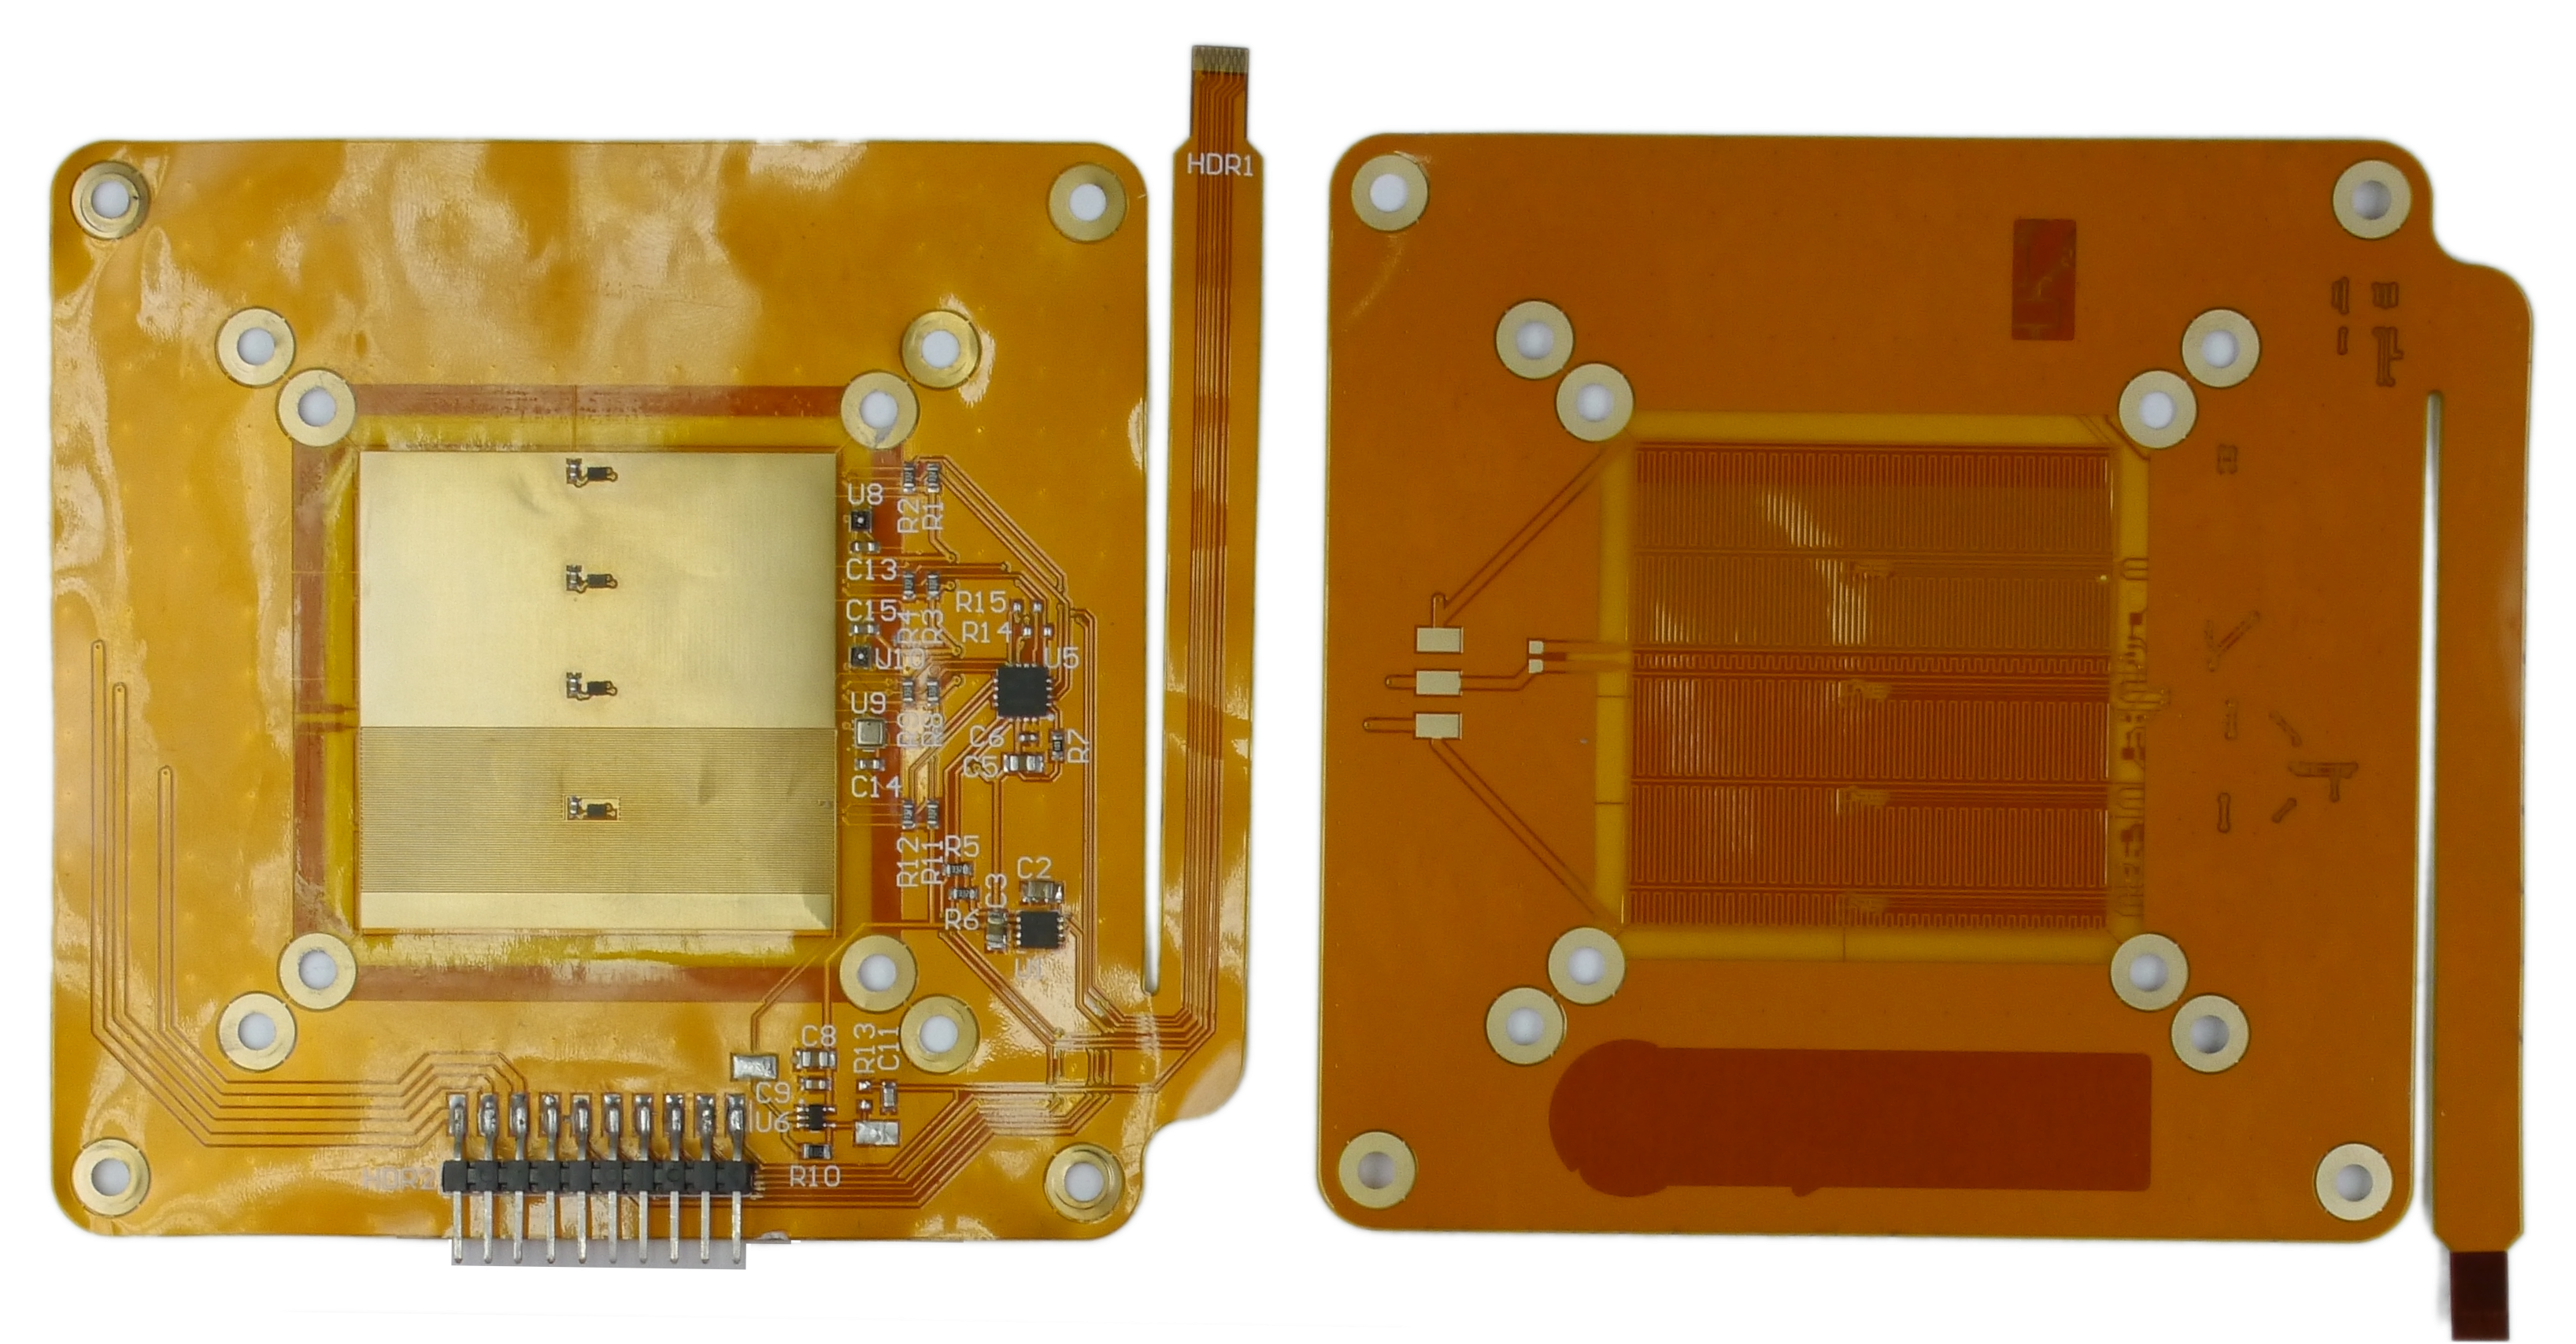
\includegraphics[width=0.9\linewidth]{images/sensor_flex1.jpg}
    \caption{Photograph of the mirror/capacitor \gls{FPC} front and back.}
    \label{i:sensor_flex}
\end{figure}

\begin{figure}[ht!]
    \centering
    % \hspace*{\fill}
    \includegraphics[width=0.9\linewidth]{images/sensor_rigid1.jpg}
    \caption{Photograph of the base \gls{PCB} alongside the STM32 microcontroller \gls{FPC}.}
    \label{i:sensor_rigid}
\end{figure}

\section{Control software}\label{c:control}
As explained in \cref{s:background,s:concept}, the measurement of the measurement principle of the chilled dew point hygrometer requires a cooling of the sensed mirror/capacitor surface.
In order to guarantee correct measurement of the dew point, an algorithm for controlling the sequence of measurement steps is therefore inevitable. As the cooling needs to be performed for a wide variety of temperature ranges and possibly requires a large change in temperature, there is a need for an estimation of the dew point temperature. Without such analysis, the measurement and energy consumption is either excessive in the case of cooling down to the lowest temperatures feasible, or otherwise potentially not sufficient, if the target temperature or cooling duration is not sufficient for reaching the dew point.
The exact analysis of dew point however is performed on an external computer after completion of the measurement cycle with methods described in \cref{c:readout}.

The software for performing the measurement cycle is written stm32duino, a software platform implementing the Arduino API for the STM32 microcontroller platform. Only a minor fraction of the code makes direct use of the officially provided hardware abstraction layer from STMicroelectronics in order to access certain hardware timer functionality. This yields the benefit of fast prototyping and cross-manufacturer compatibility requiring only minor code changes for adaption in different microcontrollers.
\clearpage
\begin{wrapfigure}{r}{0.5\textwidth}
    \centering
    \def\svgwidth{0.365\textwidth}
    \input{drawings/control2.pdf_tex}
    \caption{Control sequence}
    \label{d:control}
    \vspace{-55pt}
\end{wrapfigure}

The initiation of a measurement is performed using a host computer connected over a serial connection to the STM32 microcontroller. Different commands are provided for enabling and disabling sensors, for performing sensor readouts and most importantly for initiating the measurement cycle as seen in \cref{d:control}.

The cycle starts by setting initial conditions, such as the sensing period, the amount of repetitions and the desired temperature slopes. This leads to the entering of the control loop, which is periodically performed according to the set period. The loop first disables both cooling and heating \gls{PWM} outputs. This step is performed in order to avoid the possibility of noise introduction, especially in measurement of the capacitance, due to switching of the half bridge \glspl{MOSFET} and ripple within the \gls{TEC} and heater. 

After that, all measurements on the provided list of enabled sensors are initiated, in a parallel manner for the temperature as well as reference humidity and pressure sensors and in a sequential manner for optical and capacitive sensors. This distinction is required in order to avoid mutual interference. The complete measurement time depends on the amount and type of enabled sensors and can be expressed as 
\begin{align*}
    t_{meas} = \max \{ &\max \{t_{temp}, t_{press}, t_{hum}\}, \\
    &t_{cap} + \sum t_{prox} \}
\end{align*}
The sensors are set to measure with maximum precision wherever possible, leading to measurement times of \qty{36}{\ms} for the temperature sensors, \qty{5}{\ms} and \qty{7}{\ms} for the VCNL36825T and VCNL4040 proximity sensors, and up to \qty{10}{\ms} for the capacitor sensor. The measurement times for reference humidity and pressure sensors are in the range of \qty{10}{\ms}.

After the measurement is finished, the \gls{PWM} is turned back on and the data of the sensors is fetched. Based on the current state, the next state is determined. The state changes, if either a temperature or a capacitance limit has been reached and subsequently the temperature slope, a term of $\Delta T / s$, is updated. In the first iteration of the loop, the lower and upper boundaries for capacitor values are determined by a percentual factor of the initially measured capacitance. This is needed, in order to limit the cooling and heating duration as described above. \Cref{c:results} describes the governing physi-chemical mechanisms used for this. The temperature limits for reheating and recooling are set after the dew point was detected for the first time using the relative capacitance term.

In the following step, the temperature setpoint is determined using the actual setpoint and the offset defined by the slope. Using the temperature error, defined by the difference of measured temperature and the setpoint, the pulse width of the \gls{PWM} signal is updated by a control loop mechanism in form of a \gls{PID} controller. The controller determines a set value using the following terms:
\begin{itemize}
    \item Proportional: Produces and output value that is proportional to the current error value.
    \item Integral: Accumulates past errors over time to eliminate offset and steady-state errors.
    \item Derivative: Uses the rate of change of the error in order to accelerate the response in an abrupt system change and oscillations.
\end{itemize}
The heater was not provided with a seperate PID controller, as it only serves as a supporting system, that limits the amount of condensation on the sensor and thus decreases the time required for evaporation of dew. Its value is determined relative to cooler PID controller and is only applied in a reheating state.

The resulting pulse widths are set accordingly and all relevant data is transmitted to the host computer for dew point analysis and logging purposes. Among this data is every sensor reading, as well as the current state, temperature setpoints and errors and \gls{PID} controller values.

Finally, the state machine either proceeds with the next loop iteration after a delay of the remaining duration of the measurement period, or it finishes operation, if the last state is completed.

%Diagram exemplary response

\section{Data readout}\label{c:readout}

In the field of signal analysis, the selection of data filtering is crucial as high frequency noise can significantly impact the identification of points of interest, particularly in the presence of hard short term flanks. This issue becomes even more critical when numerical derivations need to be performed. While a linear interpolation of the original samples can be visually categorized in terms of trends, digital processing using linear interpolations of numerically derivated samples may be impossible due to abrupt changes in the slopes. To address these challenges, a variety of filters and regression techniques exist, such as finite impulse response (FIR) filters, infinite impulse response (IIR) filters, and polynomial regression methods like smoothing splines or LOESS. Commonly used filters are finite impulse response filters, which are a class of low pass filters that reduce high frequency noise. Notable implementations of FIR filters include simple moving average and weighted moving average. In a simple moving average, all samples of a filter are equally weighted using a boxcar function (also referred to as a rectangle window). In contrast, a weighted moving average assigns different weights to parts of the window, giving them higher importance. However, these filters are rather inflexible and need to be tuned accordingly. Large window sizes lead to overdampening, making it impossible to detect edges, while small values are ineffective at counteracting noise. Additionally, response time is severely slowed down and behavior at the start and end of measurement differs. 

For these reasons, a regression method, specifically smoothing splines, was chosen for this study with the primary intent to obtain reliable results in numerical derivation. For regression, a large variety of functions and approximation methods have been studied. A very versatile approach is the use of piecewise connected polynoms of a specified degree $k$, also called B-splines. For an array of $n$ samples, B-splines are globally continuous up to the $(k-1)$th derivative and defined by coefficients and knots. The coefficients are used in conjunction with localized polynomials, also called basis elements, which the B-spline is made up of:

\begin{equation}
    s(x) = \sum_{i=-k}^{n} c_i  N_{i, k}(x)
\end{equation}

The set of basis elements $\{N_{i,k}\}^n_{i=-k}$ are associated to the knot vector $T = \{t_{-k}, t_{-k+1}, ...,\\t_{n+k+1}\}$, consisting of a knot at each sample and additionally introduced boundary knots, and defined recursively by the Cox-de-Boor formula:

\begin{subequations}
    \begin{align}
        N_{i, 0}(x) &= \begin{cases}
            1,& \text{if } t_i \le x < t_{i+1} \\
            0,& \text{otherwise}
        \end{cases}\\
        N_{i, k}(x) &= \frac{x - t_i}{t_{i+k} - t_i} N_{i, k-1}(x)
        + \frac{t_{i+k+1} - x}{t_{i+k+1} - t_{i+1}} N_{i+1, k-1}(x)
    \end{align}
\end{subequations}

The formula shows, that the basis elements are linear combinations of usual monomials $x^m$  with $m = 0, 1, ..., k$ with the special feature, that they equal to zero outside an interval defined by a knot array consisting of $k + 2$ knots.
    
The amount and placement of knots defines the fitting of the curve, i.e. for the maximum amount of $n + 2k + 1$ knots, the spline completely satisfies the input array, resulting in a polynomial interpolation. In order to find a spline, i.e. its knots and coefficients, that fits the data with a variable amount of smoothing, the algorithm proposes a scheme, where the discontinuities in the $k$th derivative are to be minimized:
\begin{equation}
    \sum_{r=k+2}^{n-k-1} \left[ s^{(k)}(t_r + 0) - s^{(k)}(t_r - 0) \right]^2,
\end{equation}

while an error constraint with a passed smoothing parameter $s$ is fulfilled:
\begin{equation}
    \sum_i \left[ w_i (g(x_i) - y_i)\right]^2 \leqslant s.
\end{equation}

For a smoothing parameter equal to zero, each knot has to be traversed, leading to a high amount of discontinuities in the derivative, whereas for a sufficiently large smoothing parameter, the amount of knots will be minimal, possibly leading to an approximated curve in the form of a straight line.

In order to make use of this powerful tool, the implementation provided by the scientific computation library scipy was chosen for dew point analysis.
\chapter{Results \& Discussion}\label{c:results}
In the following sections, parts of the sensor subsystems are analyzed and the results obtained from dew point measurement shown and discussed. 

\section{Sensor subsystems}


\subsection{Temperature readout}

The temperature readout is among the most critical parts of the sensor system, as the temperature has to be determined as an absolute value with sufficient accuracy. Hence, an early test was the evaluation of multiple temperature sensors to evaluate suitable candidates for usage on the platform. Besides accuracy, critical parameters are also defined to be drift and response time, as the measurement principle requires correctness over an extended time period as well as a sufficiently fast response to temperature gradients.



The first sensor board included tests over five different temperature and ambient conditions sensors. It was performed using a Fluke 5615 \gls{SPRT}, specifying an accuracy of \qty{\pm 0.012}{\celsius} and an extremely low drift of \qty{\pm 0.007}{\celsius} at the triple point of water (\qty{0.01}{\celsius}). Therefore, its specified accuracy is approximately an order of magnitude higher than that of the tested integrated temperature sensors and hence it may be used as a reference for accuracy measurements. For the temperature control, a Fluke 7320 calibration bath was used, inside which the temperature sensors were submerged in a low viscosity silicon oil. This allows for very fine control and uniformity in temperature within the measurement environment. 

\begin{wrapfigure}{r}{0.55\textwidth}
    \centering
    \includegraphics{graphs/tempsensors_stability.pdf}
    \caption{Long duration test of temperature sensors at \qty{27}{\celsius}.}
    \label{g:temp_stability}
\end{wrapfigure}
The readout of the temperature sensors was performed in cycles of \qty{200}{\ms} using a microcontroller, which sent its data to a host machine. The \gls{SPRT} was measured using 4-wire measurement on a Keysight 3458A multimeter in order to eliminate voltage drop on the lead wires and the data was fetched over serial communication in the same frequency as for the integrated temperature sensors. The conversion from resistance to temperature was performed using the supplied ITS-90 calibration coefficients, which were specified around 2.5 years prior to measurement and state an uncertainty of around \qty{\pm 10}{\milli\kelvin} at \qty{0.01}{\celsius}. Although the drift is not specified in datasheet, it is assumed to be as low as \qty{\pm 1}{\milli \kelvin} per year, as related studies show \autocite{tavenerPlatinumResistanceThermometers2013}. The accuracy of the resistance measurement of the multimeter is stated with approximately \qty{\pm 15}{ppm} for the respective range of \qty{100}{\kilo\ohm} and the calibration period of two years, resulting in a temperature deviation of less than \qty{5}{\milli \kelvin}.

\begin{figure}[t!]
    \centering
    \includegraphics{graphs/tempsensors_dev.pdf}
    \caption{Temperature deviations for each sensor compared to the \gls{SPRT}.}
    \label{g:temp_dev}
\end{figure}

\Cref{g:temp_stability} shows the deviations during a long duration measurement of 30 minutes. The sensors used for the test were primarily the later used ams-OSRAM AS6221, Silicon Labs Si7051 and Analog Devices ADT7422. Although two samples of each sensors were intended to be tested, a mechanical failure led to one AS6221 sensor to be dismissed in the analysis. Two results of two additional humidity and temperature sensors (Texas Instruments HDC1080JS and Sensirion SHT31) have been included as well. The results show the mean temperature measurement of each sensor, as well as the standard deviation. As expected, the \gls{SPRT} showed the smallest amount of variation with around \qty{\pm 3}{\milli\celsius}. While the HDC1080JS follows right after that with around \qty{\pm 8}{\milli\kelvin}, it has the largest deviation in the absolute measurement, indicating less trueness. Hence, for this test the AS6221 sensor is determined to be the most accurate among the sensors, as it is closest to the measurement of the \gls{SPRT} while showing relatively low variations.

Another test is shown in \cref{g:temp_dev}, comparing the sensors over a range of different temperatures. For each sensor and temperature, 20 samples were taken and their mean value compared against the reference temperature reading of the \gls{SPRT}. Again, the AS6221 showed the least deviation with a maximum of \qty{-35}{\milli\celsius} at \qty{0}{\celsius}.

Besides the superior performance in temperature measurement, the AS6221 sensor also exhibits the lowest response time after a rapid change in temperature. This can be explained by its low thermal mass, as it is the smallest sensor of all, with a footprint size of \qtyproduct{1 x 1.5}{\mm}.


\subsection{Temperature control}
The temperature control is another important subset of the humidity sensor. A precise control is necessary in order to avoid measurement inaccuracies due to oscillation in temperature or changing temperature gradients.

The performance is mainly decided by two factors, the buck converter being able to supply sufficient power for the \gls{TEC} and the \gls{PID} controller, which is governing the output voltage of the buck converter.

The buck converter was designed with high current application in mind. It uses rather large \qty{330}{\milli\henry} inductance rated for \qty{3.5}{\ampere}, thus requiring \qtyproduct{12.5 x 12.5}{\mm} \gls{PCB} area. Due to the high inductance however, switching frequencies can be limited to less than \qty{200}{\k\Hz} without large sacrifices in terms of ripple, limiting the dissipated heat of the device. During tests it was found, that the buck converter is capable to provide sustained currents as high as \qty{3.5}{\A} at around \qty{14}{\V}, which is sufficient for a temperature difference of \qty{40}{\celsius}.

\begin{figure}[!b]
    \centering
    \includegraphics{graphs/pid_offset.pdf}
    \caption{Comparison of set temperature and measured temperature in a simulated dew point measurement scenario.}
    \label{g:pid}
\end{figure}

The \gls{PID} controller uses proportional, integral and derivative error terms for feedback as explained in \cref{c:implementation}. In order to find a suitable initial set of coefficients, the Ziegler-Nichols method was used. It is an heuristic approach, using the period of oscillations in a purely proportianally controlled system in order to define the integral and derivative terms. From there on, further manual adjustments have been made to optimize the performance. Main concern for the system is a high degree of linearity in order to avoid unstable dew formation and noise in temperature measurement. \Cref{g:pid} shows a resulting temperature control in an environment with starting conditions of \qty{10}{\celsius}. Beginning from t = \qty{4}{\s}, the temperature slopes have been set to \qty[per-mode=fraction]{-1.3}{\celsius\per\s} until \qty{-10}{\celsius} is reached, \qty[per-mode=fraction]{0}{\celsius\per\s} for \qty{23}{\s}, \qty[per-mode=fraction, retain-explicit-plus]{+1}{\celsius\per\s} until \qty{0}{\celsius} is reached, \qty[per-mode=fraction]{0}{\celsius\per\s} for \qty{21}{\s} and \qty[per-mode=fraction]{-0.4}{\celsius\per\s} for \qty{94}{\s}. The measured values follow the setpoint line closely, with very little difference in terms of slope. Only in case of a rapid change in the temperature set point slope, there is a clearly visible oscillation. To avoid these oscillations, the system would require either a decrease in the integral term or an increase in the derivative term, however, this would come at the cost of increased offsets, or respectively oscillations, during constant slope operation.


\subsection{Optical and capacitive readout}
The optical and capacitive readout need to reliably measure the presence of dew on the surface. In contrast to the temperature sensor, the measure quantity does not need to be detected as an absolute value, e.g. as gram or volumetric ratio, but as a relative value compared to the initial state of the system. Hence, most important factors of the dew detection are considered to be sensitivity and noise behaviour.

\subsubsection{Capacitor}
The sensitivity of the capacitive readout is first and foremost limited by the resolution of the frequency measurement of the capacitor, given that a change in capacitance is detected by the charging and discharging time of the component. This results in a proportionate relation to the product of the charge-discharge period and the sampling frequency. In the context of the measurement system, this means, the resistor governing the current and thus the period needs to be sufficiently large, while sampling with a high frequency. 

The used values were set to  \qty{1}{\mega\ohm} for the resistor and \qty{170}{\mega\Hz} for the frequency, being the maximum possible frequency for the microcontroller. The value of the capacitor was determined to be around \qty{180}{\pico\F}. At operating voltages of \qty{3.3}{\volt} for the supply voltage and measured threshold voltages of \qty{1.05}{\volt} and \qty{1.55}{\volt}, this results in a period of $T_{RC} = \qty{115.34}{\us}$ or a frequency of \qty{8.67}{\kilo\Hz} using \cref{e:cap_period}, given standard ambient conditions and neglecting stray capacitances. With a sampling period of $T_{s} = \frac{1}{\qty{170}{\mega\Hz}} = \qty{5.88}{\ns}$, this results in a sensitivity of around \qty{51}{ppm}. 

However, this high amount of sensitivity is severely limited by noise introduced into the measurement system. The noise sources affecting the system are countless, among these are:
\begin{itemize}
    \item fluctuations in supply voltage
    \item fluctuations in threshold voltage
    \item fluctuations in sampling frequency
    \item electromagnetic interference
    \item temperature
    \item mechanical forces
\end{itemize}

\begin{wrapfigure}{r}{0.5\textwidth}
    \centering
    \includegraphics{graphs/noise_cap.pdf}
    \caption{Noise analysis of capacitor readout.}
    \label{g:noise_cap}
\end{wrapfigure}
Some of these influences may be minimized by design or changes in the measurement environment, while others are given. Noise estimation is a rather difficult task due to measured size, i.e. water concentration in close proximity to the surface, being noisy. \Cref{g:noise_cap} shows a \gls{FFT} of a measurement cycle with a duration of 10 minutes, with samples taken every \qty{200}{\ms}. At higher frequencies, the Fourier transform looks flat, resembling the power spectrum of white noise, while the frequency response in the lower section follows a pink noise pattern. The measurements were conducted in controlled conditions, which were yet not completely constant with an approximately linear change in temperature of \qty[retain-explicit-plus]{+50}{\milli\celsius} and a relative humidity change of \qty[retain-explicit-plus]{-0.05}{\percent}, as measured using four temperature and three humidity sensors. The measured frequency of the Schmitt trigger circuit exhibits a response closely following the linear trend detected by the other sensors, with the frequency rising linearly from \qtyrange{6270}{6290}{\Hz}.

High noise influences on the measurement are evident however when the \gls{TEC} is powered during sensing of the capacitor, with standard deviations one order of magnitude higher than without, rendering reliable capacitance measurements infeasible. Therefore during all capacitive measurements, the \gls{TEC} is turned off. Furthermore, the capacitive readout uses 20 samples, in order to determine and remove outliers, and uses an average of the remaining values in order to reduce the impact of high frequency noise.


\subsubsection{Optical readout}
The optical readout relies on the precision of the used proximity sensors. Both are specified to detect objects within a range of \qty{20}{\mm}, yet their difference different light source leads to a different output code for a given distance. The configuration of the sensors has been set such, that their output uses as much of the scale as possible. The VNL36825T, employing a laser that emits a much narrower beam of light, uses nearly the full scale of 16 bit, with values ranging between 40000 and 60000 during the performed humidity measurements. The VCNL4040 sensor is only able to provide values that are a factor 10 lower.

\begin{figure}[!hb]
    \centering
    \begin{subfigure}{.5\textwidth}
      \centering
      \includegraphics{graphs/noise_prx1.pdf}
      \caption{VCNL4040}
      \label{g:noise_prx1}
    \end{subfigure}%
    \begin{subfigure}{.5\textwidth}
      \centering
      \includegraphics{graphs/noise_prx2.pdf}
      \caption{VCNL36825T}
      \label{g:noise_prx2}
    \end{subfigure}
    \caption{Noise analysis of the two center proximity sensors.}
    \label{g:noise_prx}
\end{figure}


\section{Humidity measurements}

\subsection{Test setup}
The hygrometric measurements were performed within an environment where conditions were regulated to maintain maximal stability. This required careful considerations for the test setup, which was established as seen in \cref{d:test_chamber}. 

The desired temperature conditions were achieved using a temperature test chamber, which is roughly sealed with some cables leaving a millimeter-sized gap to the outside. Inside the test chamber, a sealed box is placed, which is prepared with thoroughly sealed cable glands. This box contains the hygrometer, which is placed on top of a perforated plate. Below the perforated plate is a screw glass containing the reference humidity solution. For proper air exchange, such that the desired humidity can easily be reached, a fan has been put on top of the glass. For cooling of the peltier element, a heatsink and another fan was used.

\begin{figure}[h]
    \centering
    \input{drawings/test_setup.pdf_tex}
    \caption{Test chamber setup.}
    \label{d:test_chamber}
\end{figure}

The tests have been performed for three temperature and four saturation vapor pressure setpoints, which are defined by the respective substance as seen in \cref{t:equi}. The substances are mixed with water such that the water is saturated, with sufficient amount of the unsolved substance being able to draw moisture from the air. In order to reach saturation for a given temperature, the test chamber was first set to the respective target temperature with a maximum deviation of \qty{\pm0.1}{\celsius} as measured by the integrated temperature sensors. If the temperature conditions were stable, there was a settling period of \qtyrange{2}{3}{h} in order to guarantee saturation. The state was also observed using the reference humidity sensors such that no significant changes in relative humidity were observable. The sensor was tried to be left without modification, however due to increased requirements for cooling at lower temperatures, the thermal paste connecting the heatsink to the \gls{FPC} was replaced, leading to differences in absolute values of measured frequency and light. As the dew point is performed using relative changes, these changes are assumbed to be minor in terms of humidity detection. The measurements performed using the changed conditions are indicated by an asterisk at the respective rows of \cref{t:equi}.

% \begin{wraptable}{l}{1\textwidth}
\begin{table}
        \centering
    \begin{tabular}{r|ccccc|c}
        \toprule
        \toprule
    Substance                        & T [\unit{\celsius}] & RH [\unit{\percent}] & Deviation & AH [\unit{\g\per\m^3}] & p [\unit{\hecto\Pa}] \\
    \midrule
    \multirow{3}{*}{MgCl\textsubscript{2}}           & 10          & 33.47                      & \textpm 0.24 &       3.16 &       4.13 & *\\
    & 25          & 32.78                      & \textpm 0.16 &       7.59 &      10.44  & *\\
    & 40          & 31.60                      & \textpm 0.13 &      16.23 &      23.45  & \\
    \midrule
    \multirow{3}{*}{Mg(NO\textsubscript{3})\textsubscript{2} * 6H\textsubscript{2}O} & 10          & 57.36                      & \textpm 0.33 &       5.42 &       7.08  & *\\
    & 25          & 52.89                      & \textpm 0.22 &      12.25 &      16.85  & \\
    & 40          & 48.42                      & \textpm 0.37 &      24.87 &      35.94  & \\
    \midrule
    \multirow{3}{*}{NaCl}            & 10          & 75.67                      & \textpm 0.22 &       7.15 &       9.34  & *\\
    & 25          & 75.29                      & \textpm 0.12 &      17.43 &      23.99  & \\
    & 40          & 74.68                      & \textpm 0.13 &      38.35 &      55.43  & \\
    \midrule
    \multirow{3}{*}{K\textsubscript{2}SO\textsubscript{4}}           & 10          & 98.18                      & \textpm 0.76 &       9.27 &      12.12  & *\\
                                     & 25          & 97.59                      & \textpm 0.53 &      22.59 &      31.09  & \\
                                     & 40          & 96.71                      & \textpm 0.38 &      49.67 &      71.78  & \\
                                     \bottomrule
    \end{tabular}
    \caption{Equilibrium relative humidities of the substances used for measurement. Measurements performed using a change in the setup are marked by an asterisk.}
    \label{t:equi}
\end{table}
% \end{wraptable}


\subsection{Initial measurements}

\begin{figure}[h]
    \centering
    \includegraphics[width=1\textwidth]{graphs/start_range_cap_light.pdf}
    \caption{Measurements taken at the beginning of the cycle.}
    \label{g:initial_measurements}
\end{figure}

Each measurement cycle begins with a short duration for data collection in order to set thresholds based on the starting condition in order to limit cooling duration. \Cref{g:initial_measurements} shows the inital readout values at the start of the measurement cycle for each temperature as well as for each relative and absolute humidity. The circled data points were taken from a measurement before the changes on the cooling system, the rectangular data points were taken afterwards, hence any comparison between these two data series in terms of absolute values must be taken with care. Nonetheless the diagrams show a clear dependence of the initial reading on both temperature and humidity. Especially in terms of relative humidity (as seen on the left), there is a clear proportional relationship within the samples of each data series, suggesting the possibility to make qualitative predictions on relative humidity prior exact dew point determination. Correspondingly, the relation of the frequency and the absolute humidity is much less pronounced, e.g. resulting in a frequency of \textgreater\qty{7200}{\Hz} and \textgreater\qty{6200}{\Hz} for and approximate absolute humidity of \qty{20}{\g\per\m^3} at \qty{25}{\celsius} and \qty{40}{\celsius} respecively. 

With decreasing water vapor pressure however, the difference in readings between different ambient temperatures becomes less significant, with the data points being horizontally (yet also vertically) closer together at smaller absolute humidity values. This result is consistent with the behaviour of certain types of integrated capacitive humidity sensors. Chen and Jin proposed a porous $\alpha$-alumina sensor chip, which features a thin anodic-spark-deposited $\alpha$-Al\textsubscript{2}O\textsubscript{3} film with a thickness of \qty{5}{\um}, which is capable of sensing absolute humidty between dew point temperatures of \qtyrange{-80}{-10}{\celsius} and relative humidity in a range of \qtyrange{10}{95}{\percent} RH \autocite{chenAlphaaluminaMoistureSensor1992}.

The light sensors show likewise a proportional behaviour along the relative humidity values. The slopes are inverse however, possibly indicating that the photodiode of the VCNL36825T receives an increased amount of light due to the scattering.

% Capacitive sensors using porous films work on two principles of adsorption, chemisorption and physisorption. Chemisorption is a process in which a chemical reaction occurs between the surface and the adsorbate, resulting in the formation of new chemical bonds at the adsorbent surface. This process is highly selective and occurs only when a chemical connection with the adsorption site is possible; if it is, the chemisorbed complex forms the first immobile and potentially irreversible layer. As such it is also an important factor in long term drift, as the the porosity and surface area changes. In contrast, physisorption is a process in which the adsorbate and the surface remain intact and are held together by weak intermolecular van der Waals forces. The first physisorbed layer is 

\subsection{Dew point measurements}

\begin{figure}[h!]
    \centering
    \includegraphics{graphs/measurementT25RH50.pdf}
    \caption{Measurement cycle at T = \qty{25}{\celsius} and RH = \qty{52.89}{\percent}. The opaque solid lines show the temperature and the regression curve of the sensor reading respectively. The transparent lines show the derivatives of the regression curve, with the darker line being the first and the lighter line being the second derivative. The reference dew point is indicated with the blue dashed lines and the dew point detection indicated by the transparent red dashed lines.}
    \label{g:meas_cycle}
\end{figure}
The actual dew point measurements are performed as described in \cref{c:control,c:readout}. The measurement cycle is set to four decreasing and three increasing slopes with $s = \{ \qty[per-mode=fraction]{-1.3}{\celsius\per\s}, \qty[per-mode=fraction, retain-explicit-plus]{+1}{\celsius\per\s}, \qty[per-mode=fraction]{-0.4}{\celsius\per\s}, \qty[per-mode=fraction, retain-explicit-plus]{+0.3}{\celsius\per\s},\qty[per-mode=fraction]{-0.2}{\celsius\per\s}, \qty[per-mode=fraction, retain-explicit-plus]{+0.2}{\celsius\per\s},\qty[per-mode=fraction]{-0.1}{\celsius\per\s} \}$. The first decrease is used in order to set temperature targets for subsequent cooling using a percentage of the measured frequency of the capacitor as the controlling threshold. As during the first decrease in temperature, the response time of the mirror/capacitor surface is larger, as well as due to the threshold required to be set suffieciently low, there is a large error in this first realtime dew detection. This offset is compensated by adding a sufficiently large positive offset, such that the range for successive heating and cooling cycles is set to be between the detected temperature at the threshold and a positive offset of \qty{10}{\celsius}. 

\Cref{g:meas_cycle} shows an exemplary measurement cycle at an initial temperature of T = \qty{25}{\celsius} and a relative humidity of RH = \qty{52.89}{\percent}. In the following it serves as an example to describe the dew point detection algorithm. During a decrease in temperature, the measured values decrease, indicating a increased capacitance measurement for the capacitor and and an increase in scattering for the proximity sensors. The amount of the decrease per time step rises at first, although with a slight temporal offset, especially for the first period. However, at a certain point, there is a slight step in the measured curve. Here, visible amount of dew starts to form, leading to a direct change in the response of the respective sensors. The difficulty in the measurement lies in the temporal offset however. 

The capacitive sensor is much more responsive, hence the change is sensed the earliest among all sensors. The proximity sensors exhibit a certain amount of lag. Aggravating is the fact, that this temporal response is related to the slope of the temperature curve. For small changes in temperature over time, the step appears at a later moment in time and with a temperature gradient set too low, the step cannot reliably detected at all, as seen in the last period of the VCNL4040 dew point detection.

Due to this, the dew point detection of the proximity sensors has been set to an earlier point in time, namely the point, where the second derivation of the sensed value is minimal, or in other words, where the decrease in temperature accelerates most. For all sensors an additional offset of 10 samples has been chosen in order to provide guidance and to show potential benefits in further offset consideration.

\Cref{t:dew_points} show the resulting dew point values in comparison with the reference value. Due to time constraints a complete depiction over all measurements could not be performed and remains topic for further work. For the graphical representation of all measurements please refer to \cref{appendix}.

\begin{table}[]
    \begin{tabular}{|r|clllllll|}
    \hline
    Sensor     & \multicolumn{2}{c|}{Period 1}                           & \multicolumn{2}{l|}{Period 2}                           & \multicolumn{2}{l|}{Period 3}                           & \multicolumn{2}{l|}{Period 4}      \\ \hline
    Capacitor  & \multicolumn{1}{c|}{13.23} & \multicolumn{1}{l|}{10.98} & \multicolumn{1}{l|}{15.25} & \multicolumn{1}{l|}{14.41} & \multicolumn{1}{l|}{15.08} & \multicolumn{1}{l|}{14.72} & \multicolumn{1}{l|}{15.11} & 14.92 \\ \hline
    VCNL4040   & \multicolumn{1}{c|}{13.23} & \multicolumn{1}{l|}{10.98} & \multicolumn{1}{l|}{14.34} & \multicolumn{1}{l|}{13.48} & \multicolumn{1}{l|}{15.08} & \multicolumn{1}{l|}{14.72} & \multicolumn{1}{l|}{15.11} & 14.92 \\ \hline
    VCNL36825T & \multicolumn{1}{c|}{8.41}  & \multicolumn{1}{l|}{8.2}   & \multicolumn{1}{l|}{14.34} & \multicolumn{1}{l|}{13.48} & \multicolumn{1}{l|}{15.08} & \multicolumn{1}{l|}{14.72} & \multicolumn{1}{l|}{15.11} & 14.92 \\ \hline
    Reference  & \multicolumn{8}{c|}{14.72}                                                                                                                                                                                       \\ \hline
    \end{tabular}
    \label{t:dew_points}
    \caption{Measured dew points for each sensor for the example given in \cref{g:meas_cycle}.}
    \end{table}


\subsection{Discussion}
The dew point analysis is a complicated topic requiring precise measurements. \Cref{acceptable_error} shows the maximum allowed deviations in dew point measurement in order to achieve a \qty{1}{\percent} accuracy over a range of temperatures and humidities. Higher temperatures and humidities have a larger amount of acceptable error, while for high humidity measurements in low temperatures, the acceptable error becomes close to zero.  
\begin{figure}[h]
    \centering
    \includegraphics[clip, trim=0cm 0cm 0cm 1cm, width=0.95\textwidth]{graphs/dew_deviation.pdf}
    \caption{Maximum Dew Point Temperature Tolerance for a \qty{1}{\percent} accuracy}
    \label{acceptable_error}
\end{figure}
\chapter{Conclusion}
In concluding the dew point hygrometer project, the concept of dew point detection is charming, providing a visible and understandable measure of humidity. In realization however, the concept proves hard to be consequently achieved. Despite the project's inability to meet its initial goals, the experience has provided valuable insights into the complexities of designing and implementing a reliable dew point detection system. The primary difficulties encountered in this endeavor were rooted in data analysis, time constraints, and the inherent challenges of accurately detecting dew points.

While the sensors provide acceptably good readings for a change in humidity and presence of dew, the main challenge lies in the control of this complex system. The temperature ranges vary vastly, needing proper consideration for temperature gradients, cooling thresholds and periodic measurements. Even then, without properly controlled conditions, statements on the achievable accuracy are difficult to make due to changes in temperature, also induced by self-heating, and in humidity over long measurement periods.

The data readout proved to be the main and limiting challenge however. It requires careful study and analysis of correlations and even more consideration in terms of using the correct measure and offset in order to detect an accurate value for the dew point temperature.

Despite these challenges, the project has laid a foundation for future research and development in the field of dew point hygrometry. The difficulties encountered in data analysis and the constraints imposed by time have highlighted the need for innovative approaches to sensor design, data interpretation, and experimental methodology. The exploration of new materials and better control and detection algorithms, as well as the refinement of the used ones, remains a goal for future work.


\appendix
\chapter{Dew point measurements}\label{appendix}
The below figures show the dew point measurements for all described temperature and humidity ranges. The reference dew point is marked by the dashed blue line, the algorithmically detected dewpoint is shown by the red dashed line. The achieved dew point is correct, if the refernce dew temperature line, the detected dew temperature line and the the temperature curve intersect at the same point.

\begin{figure}[ht]
    \centering
    \includegraphics{graphs/t10rh33.4.pdf}
    \caption{Measurement cycle at T = \qty{10}{\celsius} and RH = \qty{33.47}{\percent}.}
    
\end{figure}

\begin{figure}[ht]
    \centering
    \includegraphics{graphs/t10rh57.4.pdf}
    \caption{Measurement cycle at T = \qty{10}{\celsius} and RH = \qty{57.36}{\percent}.}
    
\end{figure}

\begin{figure}[ht]
    \centering
    \includegraphics{graphs/t10rh75.pdf}
    \caption{Measurement cycle at T = \qty{10}{\celsius} and RH = \qty{75.67}{\percent}.}
    
\end{figure}

\begin{figure}[ht]
    \centering
    \includegraphics{graphs/t10rh98.2.pdf}
    \caption{Measurement cycle at T = \qty{10}{\celsius} and RH = \qty{98.18}{\percent}.}
    
\end{figure}

\begin{figure}[ht]
    \centering
    \includegraphics{graphs/t25rh32.8.pdf}
    \caption{Measurement cycle at T = \qty{25}{\celsius} and RH = \qty{32.78}{\percent}.}
    
\end{figure}

\begin{figure}[ht]
    \centering
    \includegraphics{graphs/t25rh52.9.pdf}
    \caption{Measurement cycle at T = \qty{25}{\celsius} and RH = \qty{52.89}{\percent}.}
    
\end{figure}

\begin{figure}[ht]
    \centering
    \includegraphics{graphs/t25rh75.pdf}
    \caption{Measurement cycle at T = \qty{25}{\celsius} and RH = \qty{75.29}{\percent}.}
    
\end{figure}

\begin{figure}[ht]
    \centering
    \includegraphics{graphs/t25rh97.6.pdf}
    \caption{Measurement cycle at T = \qty{25}{\celsius} and RH = \qty{97.59}{\percent}.}
    
\end{figure}

\begin{figure}[ht]
    \centering
    \includegraphics{graphs/t40rh31.6.pdf}
    \caption{Measurement cycle at T = \qty{10}{\celsius} and RH = \qty{31.60}{\percent}.}
    
\end{figure}

\begin{figure}[ht]
    \centering
    \includegraphics{graphs/t40rh48.4.pdf}
    \caption{Measurement cycle at T = \qty{25}{\celsius} and RH = \qty{48.42}{\percent}.}
    
\end{figure}

\begin{figure}[ht]
    \centering
    \includegraphics{graphs/t40rh75.pdf}
    \caption{Measurement cycle at T = \qty{25}{\celsius} and RH = \qty{74.68}{\percent}.}
\end{figure}

\begin{figure}[ht]
    \centering
    \includegraphics{graphs/t40rh96.7.pdf}
    \caption{Measurement cycle at T = \qty{25}{\celsius} and RH = \qty{96.71}{\percent}.}
\end{figure}


\printglossary
\printbibliography

\end{document}
